\documentclass{article}

% if you need to pass options to natbib, use, e.g.:
%     \PassOptionsToPackage{numbers, compress}{natbib}
% before loading neurips_2021

% ready for submission
\usepackage[preprint]{neurips_2021}

% to compile a preprint version, e.g., for submission to arXiv, add add the
% [preprint] option:
%     \usepackage[preprint]{neurips_2021}

% to compile a camera-ready version, add the [final] option, e.g.:
%     \usepackage[final]{neurips_2021}

% to avoid loading the natbib package, add option nonatbib:
%    \usepackage[nonatbib]{neurips_2021}

\usepackage[utf8]{inputenc} % allow utf-8 input
\usepackage[T1]{fontenc}    % use 8-bit T1 fonts
\usepackage[colorlinks=true]{hyperref}       % hyperlinks
\usepackage{url}            % simple URL typesetting
\usepackage{booktabs}       % professional-quality tables
\usepackage{amsfonts}       % blackboard math symbols
\usepackage{nicefrac}       % compact symbols for 1/2, etc.
\usepackage{microtype}      % microtypography
\usepackage{xcolor}         % colors
\usepackage[pdftex]{graphicx}
\usepackage{caption}

\title{Semantic analysis of German parliament speeches}

% The \author macro works with any number of authors. There are two commands
% used to separate the names and addresses of multiple authors: \And and \AND.
%
% Using \And between authors leaves it to LaTeX to determine where to break the
% lines. Using \AND forces a line break at that point. So, if LaTeX puts 3 of 4
% authors names on the first line, and the last on the second line, try using
% \AND instead of \And before the third author name.

\author{%
  Emanuel Fuchs\\
  Matrikelnummer xxxxxxx\\
  \texttt{emanuel-fuchs@t-online.de} \\
  \And
  Arthur Jaques\\
  Matrikelnummer xxxxxxx\\
  \texttt{arthur.jaques@live.com} \\
}

\begin{document}

\maketitle

\begin{abstract}
  We are planning to use the dataset of speech transcripts of the German Bundestag (\url{https://de.openparliament.tv/api/}).
  Our main research question is how the topics of the speeches have changed over time, both in general and by party.
  We propose to use Latent Dirichlet Allocation (LDA) for topic extraction and visualize the results both with simple barplots and time series visualizations.
\end{abstract}

\section{Introduction}

\section{Methods}
We download the texts of the Bundestag speeches in the timeframe 24 October 2017 to 7 September 2021 using the OpenParliament \cite{OpenParliamentTV} API.
We discard all speeches not attributed to any of the major parliament factions (SPD, FDP, CDU/CSU, BÜNDNIS 90/DIE GRÜNEN, AfD, DIE LINKE).
We remove as many ``formalities'' (expressions empty of content such as salutations) as possible, using regular expressions.
The resulting dataset contains 8,470 speeches
\footnote{2,101 CDU/CSU, 1,547 SPD, 1,285 AfD, 1,188 BÜNDNIS 90/DIE GRÜNEN, 1,186 FDF, 1,163 DIE LINKE.}.
207 different dates are present, and all parties held speeches in at least 91\% of them
\footnote{203 CDU, 195 SPD, 198 AfD, 193 BÜNDNIS 90/DIE GRÜNEN, 190 DIE LINKE, 189 FDP}.

For topic extraction, we use Scikit-learn's \cite{Scikit-learn} implementation of Latent Dirichlet Allocation with default parameters,  trained on the whole dataset and used to extract topics from each speech.
The features are built by stemming the texts using Nltk's \cite{Nltk} Snowball German Stemmer and vectorizing using Scikit-learn's CountVectorizer \cite{Scikit-learn}.
Tf-idf features were tried but led to less interpretable results.
After topic extraction, we analyze the words having the highest weights for each topic and try to name the topics accordingly.
We tried different parameters for vectorization and topic extraction methods (Non-negative Matrix Factorization) and decided on the parameters that yielded the best interpretable results (a subjective criterion).
In the end, we opted for 9 topics and keeping only words appearing in at least 20 speeches and at most 30\% of the total amount of speeches for vectorization.
For the visualization of time series, we use Gaussian smoothing.
To plot the average party topic distributions, we reduce the dimensionality to 2 dimensions using Principal Component Analysis.

Finally, we extract sentiments with the method provided the Python package germansentiment \cite{Germansentiment}, which uses the Bert architecture trained on German texts.
Since only a very small subset of the speeches are assigned a positive sentiment (most being neutral), we concentrate our analysis on the fraction of negative speeches.
We use p-value testing with a binomial assumption for the distribution of negative sentiments to test for significant asymmetrical differences between parties in the proportion of negative speeches.

\section{Results}
The topics extracted from the speeches dataset and the name that was assigned to them are summarized in Table~\ref{topics_table}.
\begin{table}
  \captionsetup{width=0.9\linewidth}
  \caption{Extracted topics}
  \label{topics_table}
  \centering
  \begin{tabular}{p{0.02\linewidth} | p{0.2\linewidth} | p{0.78\linewidth}}
    \toprule
    \# & Assigned name & Strongest predictors \\
    \midrule
    1 & International & europa; deutsch; russland; staat; gemeinsam; international; eu; menschenrecht; welt; turkei. \\
    2 & Military & soldat; einsatz; bundeswehr; mandat; soldatinn; mission; afghanistan; unterstutz; mali; militar. \\
    3 & EU/Economy & europa; euro; eu; unternehm; milliard; deutsch; prozent; union; geld; wirtschaft. \\
    4 & Social & kind; euro; famili; prozent; arbeit; sozial; 000; rent; miet; hoh. \\
    5 & Decisions/Law & gesetzentwurf; bundestag; glaub; fall; thema; hatt; word; entscheid; punkt; regel. \\
    6 & Democracy/Freedom & emokrati; leb; gesellschaft; freiheit; grundgesetz; staat; gewalt; deutsch; demokrat; wer. \\
    7 & German History & deutsch; wer; ost; geschicht; stiftung; abstimm; 19; opf; stimmt; bitt. \\
    8 & Ecology & klimaschutz; co; energi; prozent; erneuerbar; bau; ziel; verbrauch; energiew; wirtschaft. \\
    9 & Health/Pandemic & pandemi; schul; unternehm; arbeit; stark; digital; bass; bereich; massnahm; wirtschaft. \\
    \bottomrule
  \end{tabular}
\end{table}

\paragraph{Topics evolution in time}
An overview of the evolution of topics in the speeches is shown in Figure~\ref{stacked_area_plot}.
An analysis of single topics such as the one done in Figure~\ref{social_topic_plot} for the `Social' topic allows to examine the relative frequency of a topic in time.

\begin{figure}
  \centering
  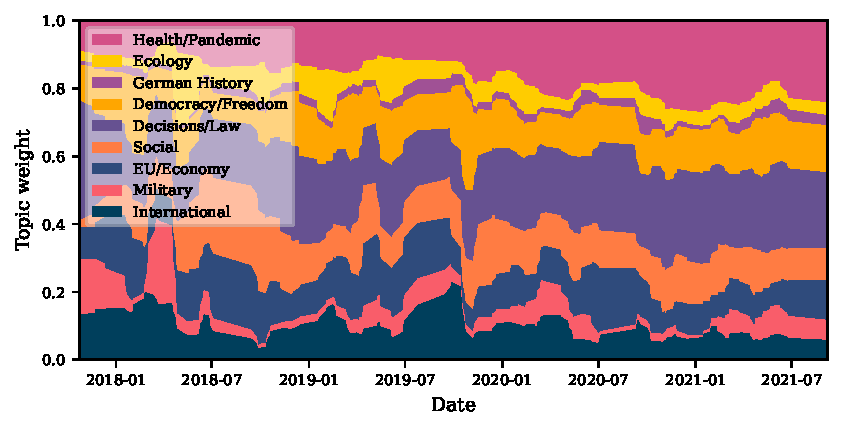
\includegraphics[width=0.9\linewidth]{images/stacked_area_plot.pdf}
  \captionsetup{width=0.9\linewidth}
  \caption{
    Average weight of topics discussed in the Bundestag (with Gaussian smoothing) between October 2017 and September 2021.
    The topics and topic weights are extracted using Latent Dirichlet Allocation.
    Notice the increased weights of both `Health/Pandemic' and `Decisions/Law' from the start of 2020 on, with the Covid 19 outbreak and consequent discussions about effective policy to tackle it.
  }
  \label{stacked_area_plot}
\end{figure}

\begin{figure}
  \centering
  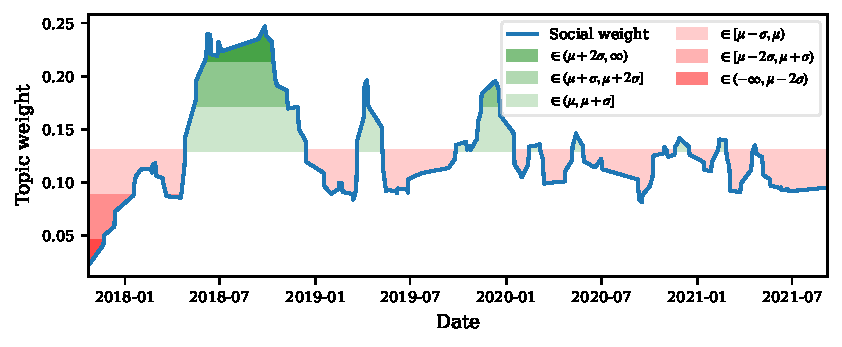
\includegraphics[width=0.9\linewidth]{images/Social.pdf}
  \captionsetup{width=0.9\linewidth}
  \caption{
    Average weight of the `Social' topic in the Bundestag speeches (with Gaussian smoothing) between October 2017 and September 2021.
    \#TODO: interpretation.
  }
  \label{social_topic_plot}
\end{figure}


\paragraph{Party topics differences}
Differences between parties can be analyzed using the same data.
In Figure~\ref{pca_plot} we show the results of 2-dimensional Principal Component Analysis on the average topic weights for each party.
The results show the parties more or less sorted on the left-right axis along the second principal component.
Furthermore, it shows the two parties that are generally considered more `extremist' (`Die Linke' and `AfD') significantly distant from the other parties.
We notice how the new `Ampel Koalition', that wasn't governing at the time, was already closer together than the governing `Schwarz-rote Koalition'.

\begin{figure}
  \centering
  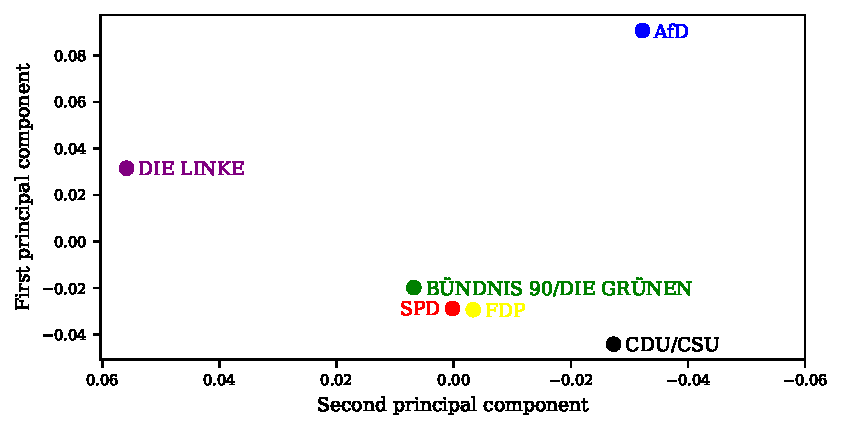
\includegraphics[width=0.9\linewidth]{images/pca.pdf}
  \captionsetup{width=0.9\linewidth}
  \caption{
    Principal Component Analysis on average topics per party.
    Notice the traditionally considered `extreme parties' at the margins, and the (at the time not governing) `Ampel Koalition' already close together.
  }
  \label{pca_plot}
\end{figure}


\paragraph{Sentiment analysis}
The extraction of sentiments from the speeches yielded in total 7,293 neutral speeches, 1,179 negative speeches, and 13 positive speeches.
Figure~\ref{sentiments_plot} shows the average sentiment (-1: negative, 0: neutral, 1: positive) by party and topic.
The plot suggests more negative speeches of non-governing parties (with `FDP' as an exception).
We performed a p-value test for significant differences between the average proportion of negative speeches over all parties and single parties.
We assumed a binomial distribution of the amount of negative speeches, and use beta-distributed priors.
We then obtained p-values for the asymmetrical differences between the whole set of speeches and the speeches of specific parties.
Using a threshold $\alpha$ of $0.05$ with Bonferroni correction for multiple testing
\footnote{2 asymmetrical tests per party and 6 parties yield 12 hypotheses, and a corrected $\alpha=0.004$}
we refuted the null hypotheses that both `SPD' and `CDU' have bigger or equal binomial coefficients of negative speeches than the Bundestag's mean,
and that `BÜNDNIS 90/DIE GRÜNEN', `AfD', and `DIE LINKE' have smaller or equal binomial coefficients of positive speeches than the Bundestag's mean.
We did not obtain significant results for both asymmetrical tests in the case of `FDP'.
These results are in principle coherent with the hypothesis that non-governing parties tend to hold more negative speeches.

\begin{figure}
  \centering
  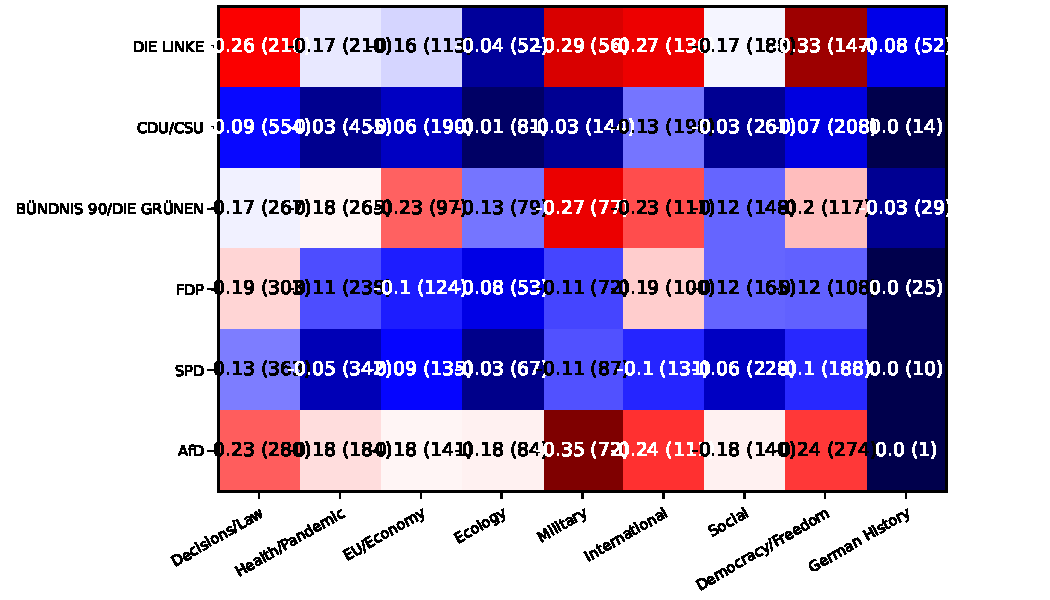
\includegraphics[width=0.9\linewidth]{images/sentiments_confusion.pdf}
  \captionsetup{width=0.9\linewidth}
  \caption{
    Average sentiment (from -1, fully negative, to +1, fully positive) by party and topic, extracted using the Python package germansentiment \cite{Germansentiment}.
    The number in brackets indicates the number of speeches the mean is constructed from, to give an idea of the significance of the number (low for example for `History' topic).
    Each speech is assigned to a single topic (the one with the highest weight).
    Notice the difference between governing and non-governing parties.
  }
  \label{sentiments_plot}
\end{figure}


\section{Discussion and conclusion}
Limitations:
\begin{itemize}
  \item Data: incomplete data, aggressive procedure to get data, reliance of data
  \item Visualization: smoothing (free parameters), short time frame, topics dictated by agenda
  \item Topic extraction: free parameters, subjectivity of chosen topic names
  \item Sentiment analysis: black-box model
  \item p-value testing: correlated hypotheses, unbalanced data, data contained in both sets
\end{itemize}

\bibliographystyle{plain}
\bibliography{bibliography}

\end{document}
